\chapter{Experimentos}
\label{cap:capitulo6}

\begin{flushright}
\begin{minipage}[]{10cm}
\emph{El único modo de hacer un gran trabajo es amar lo que haces}\\
\end{minipage}\\

Walter Isaacson, \textit{Steve Jobs}\\
\end{flushright}

\vspace{1cm}


En este capítulo se tratarán los diferentes experimentos que se han realizado para llevar a cabo este proyecto, desde las pruebas más simples hasta las más complejas, cuyo éxito ha permitido el desarrollo del software y la obtención de los resultados finales.


\section{Calibración magnética}
\label{sec:cal_mag}

Una vez obtenido el ángulo de orientación como se explica en la Sección \ref{subsec:orientacion_robot}, es necesario tener en cuenta 3 aspectos. Como vivimos en una época en la que estamos rodeados de material magnético y de campos magnéticos inducidos por los dispositivos electrónicos que nos rodean, como los teléfonos y ordenadores, es necesario eliminar las fluctuaciones que estas variables pueden provocar en este experimento.\\

\subsection{Sesgo de Hard Iron}
\label{subsec:hard_iron}

El sesgo de Hard-Iron se refiere a un tipo de error sistemático causado por la presencia de un campo magnético fijo, como el de la Tierra o materiales ferromagnéticos cercanos como piezas metálicas, imanes, dispositivos electrónicos, que pueden distorsionar las lecturas del magnetómetro. Esto se puede corregir restando un valor de compensación fijo de las lecturas del MPU9250, que se puede determinar calibrándolo en un entorno de campo magnético conocido.

Antes de empezar con la calibración, se debe asegurar que el sensor se encuentra en una superficie plana horizontal. Primero se nos pedirá rotar el sensor 360º en los 3 ejes para obtener las medidas y visualizar la respuesta magnética de los sensores del magnetómetro.

Es fácil ver la gran variabilidad entre los tres planos del sensor antes de la compensación por el efecto del Hard-Iron. La rotación de 360° del sensor alrededor de cada eje debería producir un círculo centrado alrededor del origen ya que así se demuestra que se han eliminado los sesgos y está correctamente alineado, que se aprecia después de la compensación por los efectos del Hard-Iron como se puede apreciar en esta Figura \ref{fig:hardiron}.

Los efectos del Hard-Iron primero deben restarse de los valores del magnetómetro que se están leyendo, ya que aumentará la precisión y la estabilidad de la aproximación de la orientación que se utiliza para esta aplicación de IMU.

\begin{figure}[H]
  \centering
  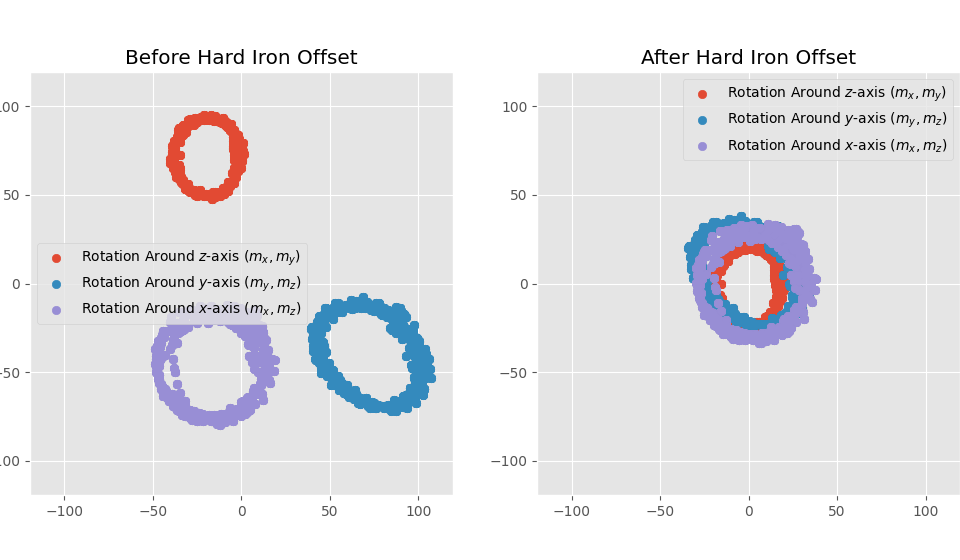
\includegraphics[scale=0.6]{figs/hard_iron_calibration} % Escala la imagen al 150% de su tamaño original
  \caption{ Representación de los efectos del sesgo de Hard Iron corregidos.}
  \label{fig:hardiron}
\end{figure} 

\subsection{Sesgo de Soft Iron}
\label{subsec:soft_iron}

Como se puede ver en la imagen, todavía hay algo de distorsión, así que se verá qué hace la eliminación del sesgo de Soft Iron.

Este sesgo es causado por la presencia de un campo magnético no uniforme, como la distorsión del campo magnético de la Tierra por objetos cercanos. Esto puede provocar que las lecturas del magnetómetro se desvíen hacia una dirección o eje particular y se puede corregir mediante un proceso de calibración que implica girar el sensor en un espacio 3D y recopilar datos del magnetómetro, que se pueden utilizar para calcular valores de corrección que se pueden aplicar a las lecturas del magnetómetro para compensar el campo magnético no uniforme.

El primer paso será guardar los datos ya calibrados previamente antes en un archivo, y se leerá de la entrada estándar, escalando así cada eje del magnetómetro obteniendo los factores de escala de cada eje para garantizar que la forma de rotación de la IMU mantenga su forma circular y si hay Soft-Iron presente, la rotación de la IMU producirá una respuesta más elíptica en lugar de circular y se obtendrán unos factores de escala los cuales habrá que multiplicar a los valores ya calibrados previamente. Como se puede ver en la Figura \ref{fig:softiron}, sigue teniendo una forma circular muy parecida por lo que se demuestra que no hay apenas Soft Iron presente, ya que sino tendría una respuesta más elíptica.

\begin{figure}[H]
  \centering
  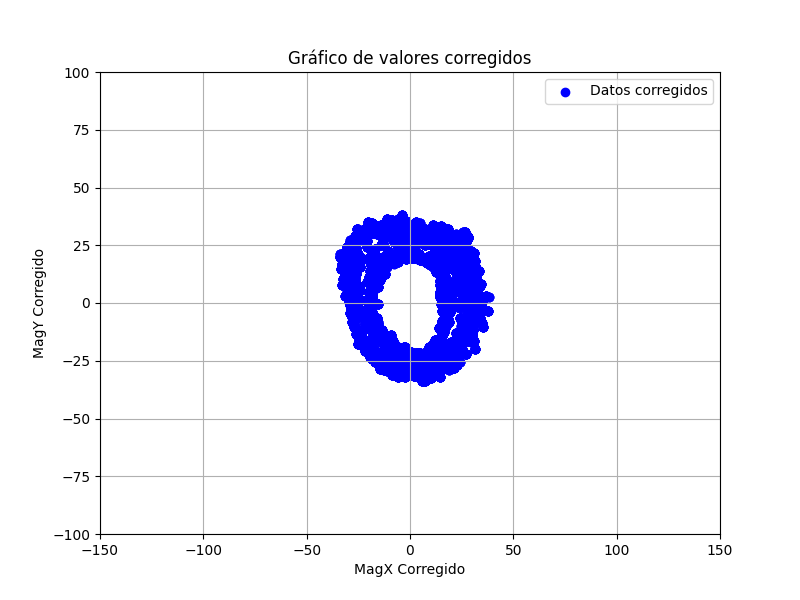
\includegraphics[scale=0.6]{figs/soft_iron_calibration} % Escala la imagen al 150% de su tamaño original
  \caption{ Representación de los efectos del sesgo de Soft Iron corregidos.}
  \label{fig:softiron}
\end{figure} 

\subsection{Filtro de paso bajo}
\label{subsec:filtro_paso_bajo}

A pesar de la calibración, todavía se pueden obtener más fluctuaciones como picos aleatorios en las lecturas magnéticas y no se busca que estas fluctuaciones nos desvíen de la señal buscada que es el campo magnético de la Tierra. Para lidiar con estos picos se implementará un filtro de paso bajo sobre los valores ya calibrados previamente con el Código \ref{cod:codejemplo5}:

\begin{code}[H]
\begin{lstlisting}[language=Python]
def low_pass_filter(valor_previo, nuevo_valor):
    return 0.85 * valor_previo + 0.15 * nuevo_valor
\end{lstlisting}
\caption[Función para aplicar un filtro de paso bajo]{Función para aplicar un filtro de paso bajo}
\label{cod:codejemplo5}
\end{code}


Como se puede ver, los pesos de este filtro suman 1 (0,85 + 0,15) y debe ser de esta manera ya que la premisa es que se confíe más en el valor anterior que en el nuevo. De esta manera se puede eliminar o reducir este ruido y mejorar la calidad de la medición de la señal del magnetómetro. Si se hubiese dado un peso mayor al dato nuevo, el filtro será más sensible a los cambios recientes, y con un peso más bajo los cambios serán más lentos pero se priorizará la estabilidad que es lo que se busca.

\section{Elección del modelo de aprendizaje automático}
\label{sec:eleccion_modelo}

Para elegir el modelo que se va a usar para entrenar a la red, hay que observar el rendimiento de cada uno de los modelos y seleccionar el más fiable para un datasets de audios. En este experimento se usó un dataset diferente que no es el mismo que se usará en la prueba final del robot, ya que al final se probará solo con varias clases y en este hay más, pero servirá para tener en cuenta la precisión de cada modelo. \\

Una vez se tienen las características escaladas como se mencionó anteriormente, es necesario usar la función específica del módulo sklearn.model\_selection \verb|train_test_split(features_scaled, directions, test_size,random_state)| para dividir el conjunto de datos en conjuntos de prueba y entrenamiento. El primer parámetro son las características una vez estén escaladas, el segundo corresponde al conjunto de etiquetas o clases asociadas a un comando de voz, el tercero representa el porcentaje que va para las pruebas (siendo el porcentaje restante para entrenamiento) y el último debe ser un número entero cualquiera para que siempre se genere los mismos subconjuntos, ya que si es \textit{None} o no se especifica, cada vez que se ejecute el código se dividirán de manera diferente y lo que se busca es que sea determinista y que no cambie con cada ejecución. El modelo se prueba en el 80\% de los datos y se prueba su rendimiento en el 20\% de los datos, que nunca ha visto en el entrenamiento. Esta función devuelve el conjunto de características para prueba y entrenamiento que es lo que se busca y también devuelve las etiquetas correspondientes a las características para entrenamiento y prueba que no se tendrán en cuenta ya que no son necesarias.\\

El siguiente paso sería evaluar los diferentes modelos de clasificación, iterando sobre cada uno de ellos, entrenando cada modelo con los datos de entrenamiento y calculando la precisión de cada uno en los datos de prueba. Como se puede apreciar en la figura \ref{fig:modelos}, se puede observar que el modelo más fiable sería RandomForestClassifier y la clasificación por vectores de apoyo SVC. Finalmente se usará el primer modelo, ya que los bosques aleatorios son modelos excelentes para utilizar como referencia debido a su baja complejidad de tiempo de entrenamiento y a su robustez frente a distribuciones desconocidas y valores atípicos en el conjunto de datos.

\begin{figure}[H]
  \centering
  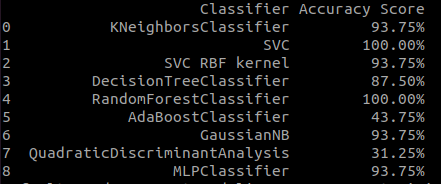
\includegraphics[scale=0.6]{figs/modelos} % Escala la imagen al 150% de su tamaño original
  \caption{ Precisión de cada modelo.}
  \label{fig:modelos}
\end{figure} 

\section{Elección del número de APs}
\label{sec:num_aps}

Para averiguar cuántos \hyperlink{APs}{APs} son necesarios para estimar la posición del robot y que haya el mínimo de error, antes es necesario probar el sistema en cuatro escenarios de prueba donde se evaluaron dos hipótesis diferentes:

\begin{enumerate}
 \item \textit{} ¿La precisión de las IPS Wi-Fi HaLow escala linealmente con el número de balizas?
 \item \textit{} ¿La precisión aumenta cuando la distancia mínima entre dos posiciones del grid es de 1 metro mientras que el área de mapeo no cambia?
\end{enumerate}\


Este experimento se probará en una habitación dividida en cuadrículas de 4x4 y se partirá de la base:

\begin{itemize}
\item \textit{} Las balizas \hyperlink{BLE}{BLE}  no se moverán de su posición durante la fase de entrenamiento y prueba.
 \item \textit{} 140 muestras por cada punto de cuadrícula son suficientes para capturar la dinámica \hyperlink{RSSI}{RSSI} (Al principio se probó con 180 muestras pero luego se probó con 140 y no cambiaban apenas los resultados).
 \item \textit{} La interferencia de WiFi y otras señales \hyperlink{BLE}{BLE}  se tendrán en cuenta.
 \item \textit{} Los escenarios de prueba realizados con 2 nodos, 3 nodos y 4 nodos son suficientes para responder a la hipótesis 1.
 \item \textit{} Para todos los escenarios, el dispositivo receptor deberá poder detectar todas las balizas WiFi presentes.
 \item \textit{} Entre cada punto del grid habrá una separación de medio metro.
\end{itemize}\


Esta imagen \ref{fig:escenario} muestra el entorno experimental para este proyecto.

\begin{figure}[H]
  \centering
  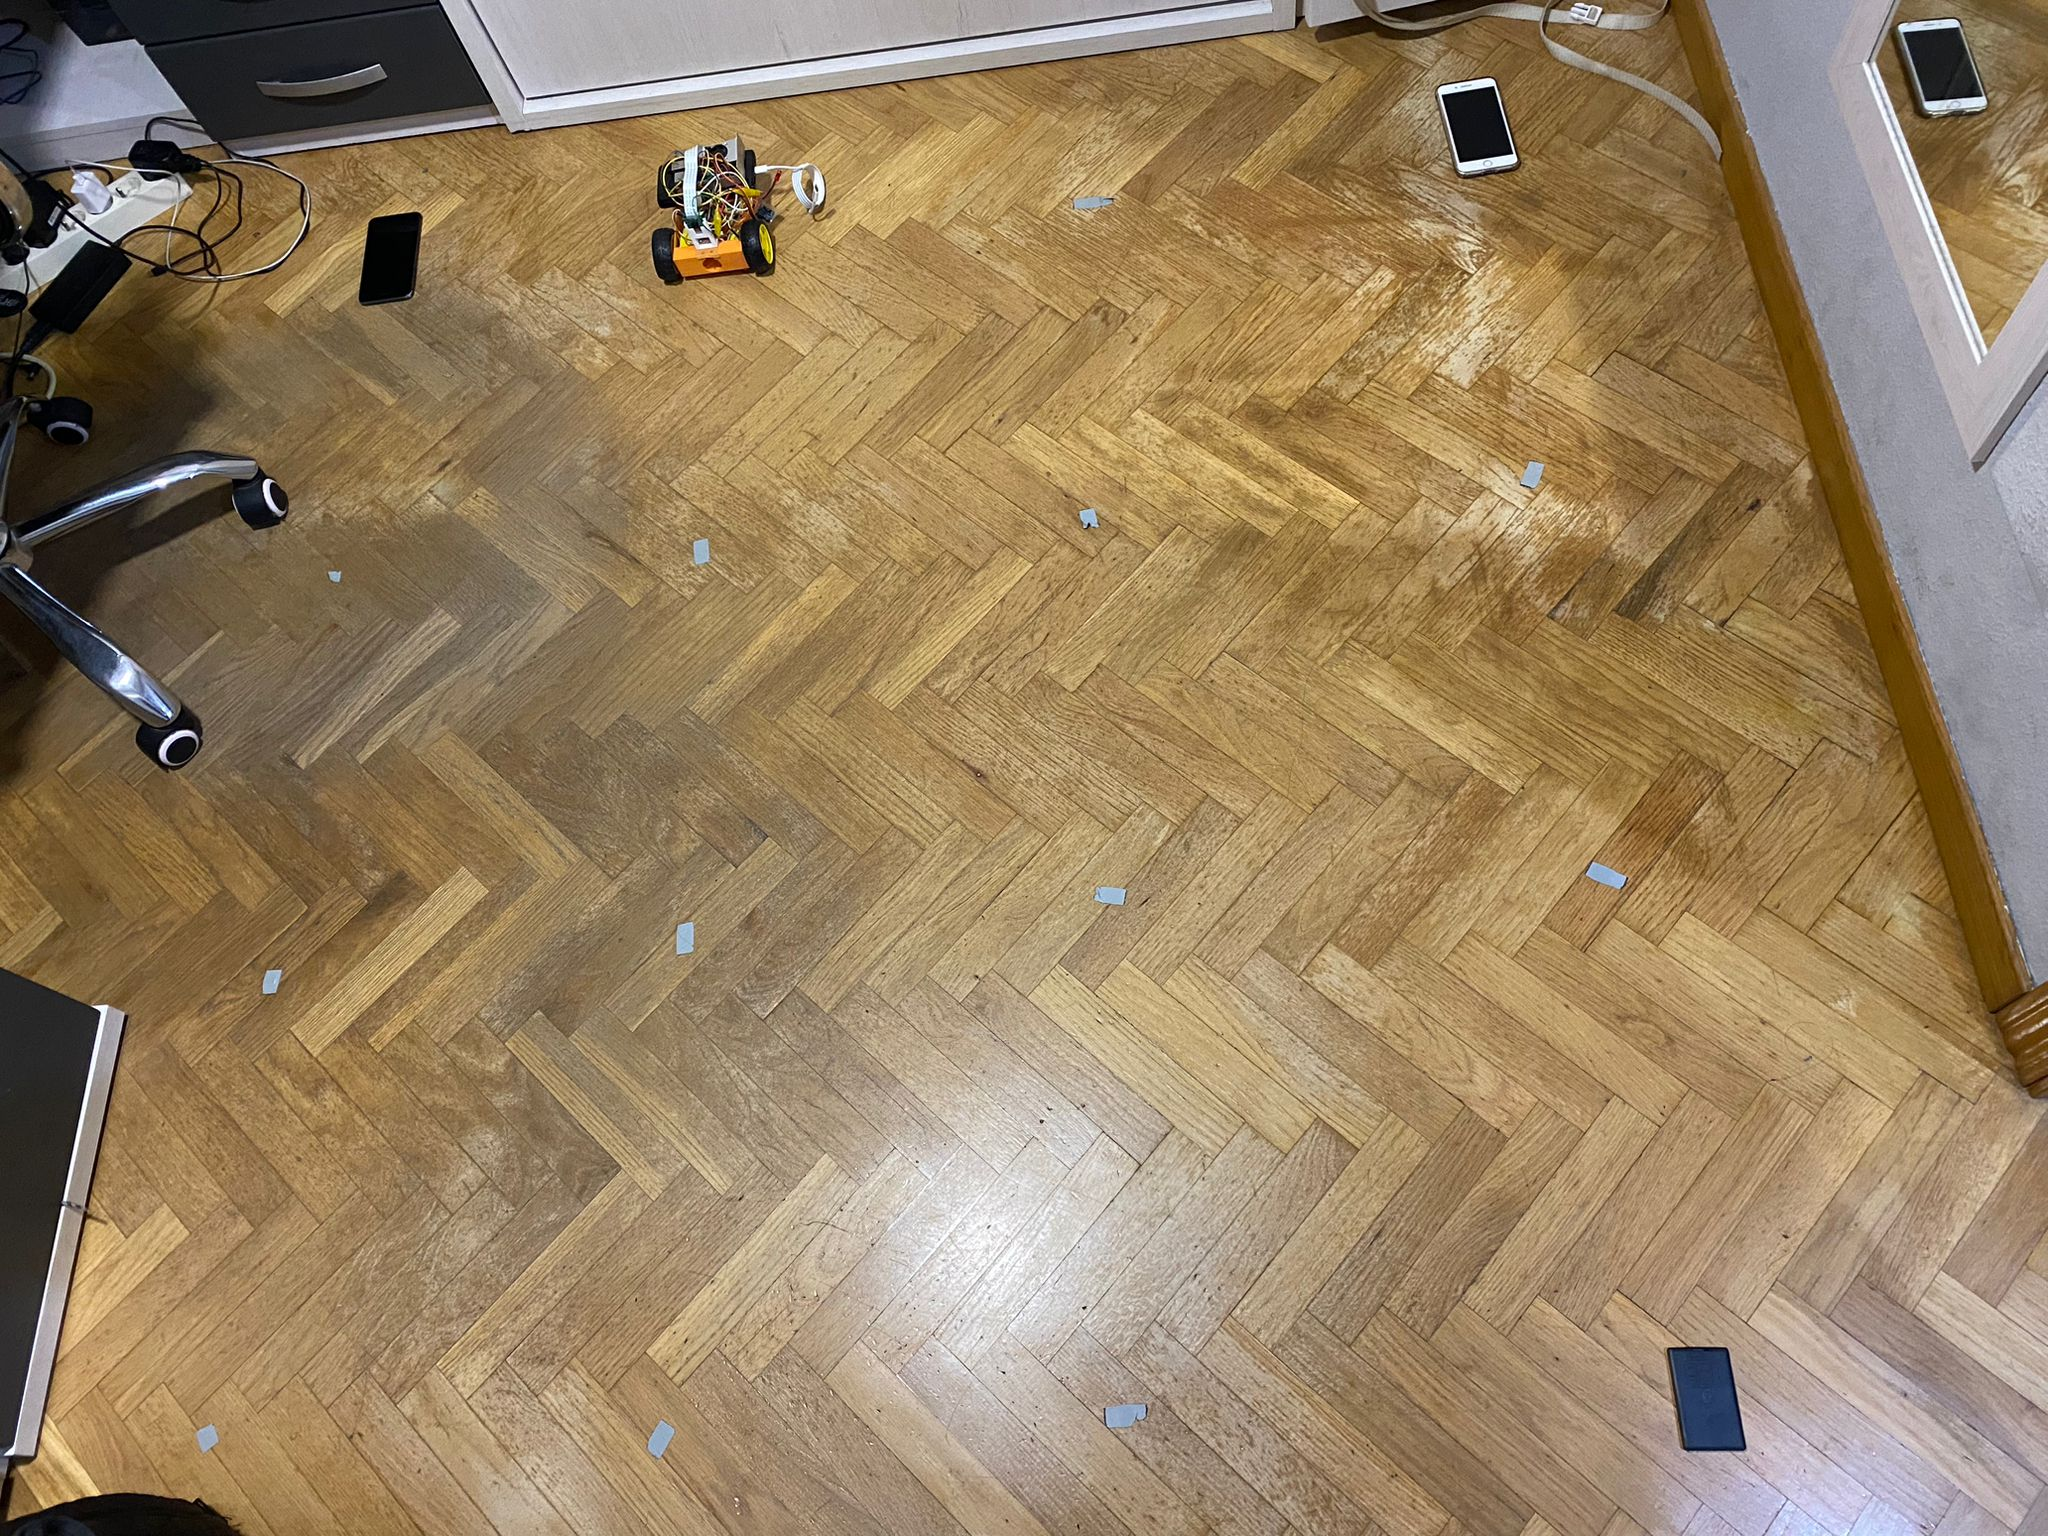
\includegraphics[scale=0.15]{figs/escenario} % Escala la imagen al 150% de su tamaño original
  \caption{ Entorno experimental.}
  \label{fig:escenario}
\end{figure} 

A continuación se mostrará los cuatro escenarios de prueba con detalles adicionales:




\begin{figure}[H]
    \centering
    % Primera fila de imágenes
    \begin{minipage}[b]{0.45\textwidth}
        \centering
    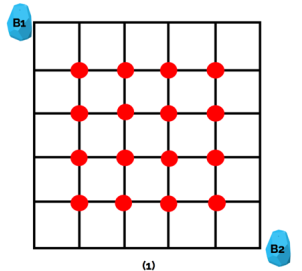
\includegraphics[width=6.5cm]{figs/dos_apes.png}
        \caption{Primer escenario de prueba}
        \label{fig:escenario1}
    \end{minipage}
    \hfill
    \begin{minipage}[b]{0.45\textwidth}
        \centering
    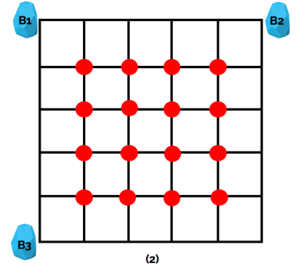
\includegraphics[width=6.5cm]{figs/tres_apes}
        \caption{Segundo escenario de prueba}
        \label{fig:escenario2}
    \end{minipage}
    
    \vspace{1cm} % Espacio entre filas
    
    % Segunda fila de imágenes
    \begin{minipage}[b]{0.45\textwidth}
        \centering
    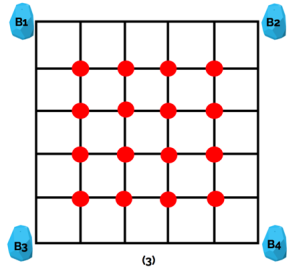
\includegraphics[width=6.5cm]{figs/cuatro_apes}
        \caption{Tercer escenario de prueba}
        \label{fig:escenario3}
    \end{minipage}
    \hfill
    \begin{minipage}[b]{0.45\textwidth}
        \centering
    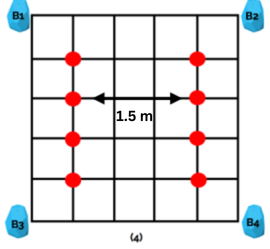
\includegraphics[width=6.5cm]{figs/cuatro_apes_espaciados}
        \caption{Cuarto escenario de prueba}
        \label{fig:escenario4}
    \end{minipage}
\end{figure}


Esta sala de pruebas se toma como un cuadrado de 1,5 metros por 1,5 metros, marcado en un piso de madera. B1, B2, B3 y B4 representan las balizas de proximidad. En este caso se elegirán modelos iPhone que, mediante la transmisión de datos móviles, se conectarán a la Raspberry y servirán como puntos de acceso.

Cada una de las marcas grises marcadas en el suelo representa un punto de la cuadrícula etiquetado del 1 al 16. Cada uno de los números ordinales marcados aquí es una etiqueta de clase que el modelo tiene que predecir después del entrenamiento con los datos recopilados.

Para entender cómo se usa esto para estimar la posición, se presenta la analogía de un “faro”. Un faro proyecta una luz de intensidad fija en el océano. Un barco puede estimar su posición relativa con respecto al faro siguiendo la intensidad del haz de luz a medida que se acerca al faro. El mismo principio es aplicable para los valores \hyperlink{RSSI}{RSSI}. Si el receptor está cerca de la baliza, el valor es mayor y se reduce progresivamente a medida que el receptor se aleja.

Después de configurar los nodos y preparar el área de experimentación, se coloca la Raspberry Pi en cada uno de los puntos de la cuadrícula gris y se recolectan 140 muestras por punto. Esta tabla \ref{cuadro:tabla1} muestra un conjunto de datos de muestra para el escenario 1.


\begin{table}[H]
\begin{center}
\begin{tabular}{|c|c|c|c|}
\hline
\textbf{Index} & \textbf{B0} & \textbf{B1} & \textbf{Label}  \\
\hline
s1 & -59 & -36 & 1 \\  
s3 & -59 & -38 & 1 \\   
s3 & -54 & -37 & 1 \\   
\hline
\end{tabular}
\caption{Ejemplo de un conjunto de datos del escenario 1}
\label{cuadro:tabla1}
\end{center}
\end{table}


Aquí, \texttt{B0} y \texttt{B1} corresponden a la posición de los nodos \texttt{B1} y \texttt{B2} que se muestran en la figura del primer escenario (Figura \ref{fig:escenario1}). En términos de la jerga del aprendizaje automático, nuestros “vectores de características” son las columnas que corresponden al valor \hyperlink{RSSI}{RSSI} de un nodo, mientras que la columna “Etiqueta” es el resultado esperado.

Después de completar la recopilación de datos, se verifican los datos en busca de valores faltantes. Se encontró que aparecían valores como \textit{None} en ciertas muestras. En estos casos, simplemente se copia el valor \hyperlink{RSSI}{RSSI} de la muestra anterior.

Los datos preprocesados se dividieron luego en una división de prueba y entrenamiento de 90\texttt{-}10. Después de eso, se aplicarán cuatro modelos de aprendizaje automático a los datos y se comparan los resultados para responder a las dos hipótesis establecidas. Los escenarios del 1 al 3 se utilizaron para responder la hipótesis 1 y, el escenario 4 se utilizó para responder la hipótesis 2.

Además, se utilizó una técnica de ajuste automático de hiperparámetros llamada GridSearchCV para buscar en el espacio de hiperparámetros de cada uno de los cuatro escenarios para obtener los mejores parámetros que se ajustan bien a los datos sin sobreajustarlos pasándole como parámetro el estimador que implementa la interfaz del estimador de scikit-learn y debe proporcionar una función de puntuación o debe pasarse la puntuación.

Ahora se probarán los diferentes modelos para cada escenario en una herramienta interactiva llamada Jupyter Notebook como ya se mencionó anteriormente en esta sección \ref{subsec:Jupyter}. Primero se probará SVC con Kernel Lineal que está basado en \hyperlink{SVM}{SVM} (Support Vector Machine) cuyo objetivo es encontrar un hiperplano óptimo que separe los datos en diferentes clases con el mayor margen posible. En segundo lugar se probará SVC con Kernel \hyperlink{RBF}{RBF} (Radial Basis Function) el cual es capaz de clasificar datos los cuales no son linealmente separables. En tercer lugar se probará con árboles de decisión los cuales dividen el conjunto de datos en función de una característica y se construyen nodos que representa la condición y las ramas que dividen los datos en subconjuntos. Por último se usará Random Forest el cual está basado en múltiples árboles de decisión y en vez de entrenar un único árbol, crea un conjunto de ellos y combina las predicciones para reducir el sobreajuste y mejorar la precisión y se obtuvieron los siguientes resultados en esta tabla \ref{cuadro:tabla2} para los escenarios 1,2 y 3 respectivamente:


\begin{table}[H]
\begin{center}
\begin{tabular}{|c|c|c|c|c|}
\hline
\textbf{Nodos} & \textbf{SVC, Linear} & \textbf{SVC,RBF} & \textbf{DTREE} & \textbf{RF} \\
\hline
2 & 28\% & 31\% & 28\% & 24\% \\  
3 & 82\% & 86\% & 78\% & 82\% \\   
4 & 94\% & 94\% & 91\% & 94\% \\   
\hline
\end{tabular}
\caption{Resultados de los modelos para los primeros tres escenarios}
\label{cuadro:tabla2}
\end{center}
\end{table}


De la anterior tabla se deduce que la precisión de los cuatro modelos aumenta a medida que aumenta el número de nodos. Por lo tanto, se concluye que la hipótesis 1 la cual planteaba el hecho de si la precisión de las IPS Wi-Fi Halow escala linealmente con el número de balizas y se confirma que es verdadera. Además, todos los modelos tuvieron un desempeño significativamente bueno en contraste con los anteriores. Sin embargo, aunque la mejor precisión es del 94\%, aunque parezca suficiente no lo es, ya que se busca el 100\% porque todo lo que no sea eso supondrá un error en la medición de la posición del robot y que por mínima que sea, puede afectar al posicionamiento del mismo.

Se atribuye este bajo número de precisión al hecho de que cada uno de los puntos de la cuadrícula está a solo 50 cm de distancia, mientras que la regla general común era separarlos entre sí por 1,5 \texttt{-} 2 metros. Esto provocó que los pares de puntos de la cuadrícula adyacentes tuvieran valores \hyperlink{RSSI}{RSSI} superpuestos, como se muestra en esta Figura \ref{fig:vals1}:



\begin{figure}[H]
  \centering
  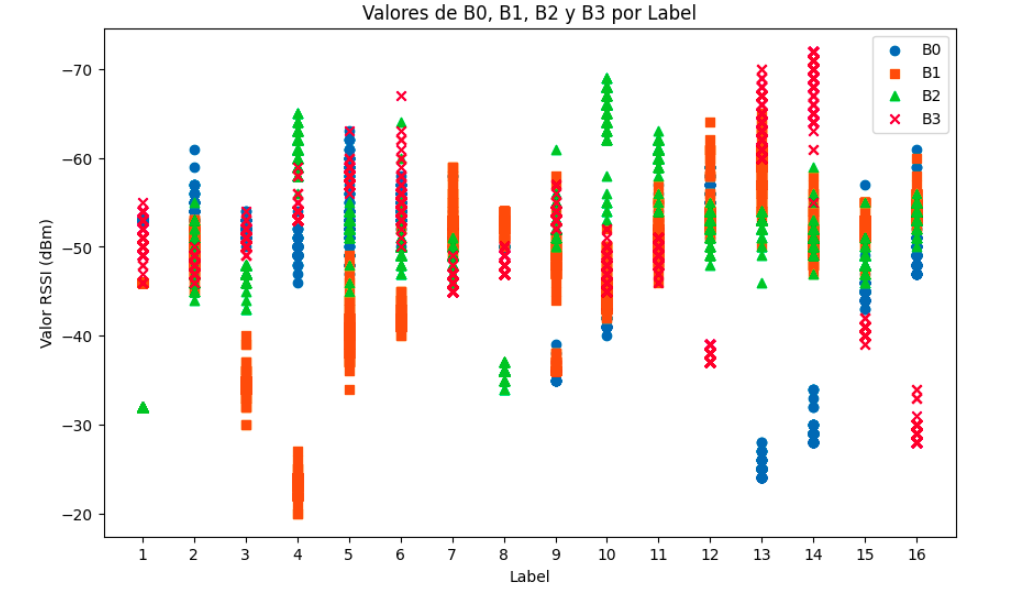
\includegraphics[scale=0.4]{figs/vals1} % Escala la imagen al 150% de su tamaño original
  \caption{ Representación de los valores RSSI en cada punto de la cuadrícula para cada AP.}
  \label{fig:vals1}
\end{figure} 

Esta tabla \ref{cuadro:tabla2} muestra los resultados del escenario 4:

\begin{table}[H]
\begin{center}
\begin{tabular}{|c|c|c|c|c|}
\hline
\textbf{Nodos} & \textbf{SVC, Linear} & \textbf{SVC,RBF} & \textbf{DTREE} & \textbf{RF} \\
\hline
4 & 99\% & 99\% & 96\% & 100\% \\  
\hline
\end{tabular}
\caption{Resultados de los modelos para el cuarto escenario}
\label{cuadro:tabla2}
\end{center}
\end{table}


Cada uno de los modelos ha demostrado obtener una mejora significativa rozando la perfección en la precisión en comparación con el escenario 3. Por lo tanto, se concluye que la hipótesis 2 la cual planteaba el efecto de separación de los puntos de la cuadrícula en la precisión de los clasificadores, es verdadera. Se justifica esta mejora señalando que, con una cuadrícula de ubicación espaciada, hubo menos superposición de datos \hyperlink{RSSI}{RSSI} entre posiciones adyacentes como se puede apreciar en esta Figura \ref{fig:vals2} y por lo tanto mayor precisión en los modelos al clasificar los datos:

\begin{figure}[H]
  \centering
  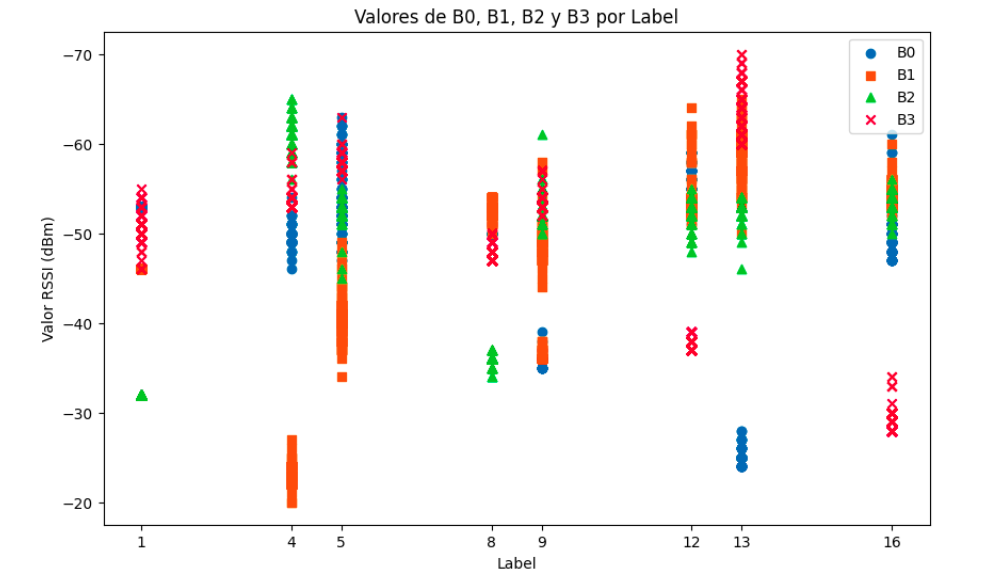
\includegraphics[scale=0.4]{figs/vals2} % Escala la imagen al 150% de su tamaño original
  \caption{ Representación de los valores RSSI en una cuadrícula espaciada para cada AP.}
  \label{fig:vals2}
\end{figure} 

En este experimento se usó la banda de frecuencia 2.4835 GHz que es de las más utilizadas para las comunicaciones inalámbricas. Al solo disponer de Iphones, no se pudo cambiar a la banda de 5GHz para transmitir y así obtener mediciones más precisas ya que esta banda tiene menos congestión y menos interferencias ya que menos dispositivos tienden a usarla, lo que mejora la calidad de la señal, mientras que la de 2.4385 GHz, tiene mayor interferencia debido a la saturación de dispositivos que la utilizan esta banda (como microondas, teléfonos inalámbricos...), lo que puede afectar la calidad de la transmisión y es más susceptible a interferencias de otras redes Wi-Fi cercanas, ya que muchas redes en un área densa suelen operar en los mismos canales.

En este experimento se ha demostrado con éxito la aplicación de un sistema de posicionamiento en interiores utilizando balizas WiFi y modelos de aprendizaje automático. Se prueban dos hipótesis y se demuestran que eran verdaderas siempre que se tuvieran en cuenta ciertos supuestos.

Por último, se ha llegado a la conclusión de que 4 \hyperlink{APs}{APs} serían suficientes para obtener una localización decente del robot como ya se demostró en la hipótesis 2. El error en el cálculo de la posición del robot respecto al centro de la cuadrícula en la que debería estar era de aproximadamente 20 cm, lo cual es una distancia razonable y útil para poder localizar al robot.


\section{Prueba final}
\label{prueba_final}



En esta sección se evalúan los factores técnicos que determinan el rendimiento
y la habilidad del robot guía. Para ello, esta prueba se ha llevado a cabo bajo distintas circunstancias:

\begin{itemize}
 \item \textit{} Las balizas \hyperlink{BLE}{BLE}  no se moverán de su posición.
 \item \textit{} La interferencia de WiFi y otras señales \hyperlink{BLE}{BLE}  se tendrán en cuenta.
 \item \textit{} Este escenario de prueba ha sido realizado con 4 nodos.
 \item \textit{} Entre cada punto de cuadrícula del mapa habrá una separación de medio metro.
 \item \textit{} Hay obstáculos de por medio en el mapa.
 \item \textit{} La red neuronal ha sido entrenada para reconocer un máximo de dos comandos de voz a diferentes distancias.
 \item \textit{} En este experimento se usó la banda de frecuencia 2.4835 GHz.
\end{itemize}\


Además, se han grabado unos vídeos que reflejan el funcionamiento del sistema. En el primer vídeo\footnote{\url{https://youtube.com/shorts/wm4-3SVO6g4?feature=share}} se aprecia como el robot va hacia el objetivo el cual se le ha transmitido por un comando de voz y en el segundo vídeo\footnote{\url{https://youtube.com/shorts/i80oPc5RJ9w?feature=share}} va hacia otra posición de la casa, dado otro comando por voz.\\

En primer lugar, para obtener los datos de los sensores que se han usado y procesarlos para su posterior uso, se han lanzado dos hilos que recogen continuamente los datos del magnetómetro y del sensor de ultrasonido, y se conforme se van leyendo, se van añadiendo a una doble cola que permita extraer el último valor y que tenga tamaño máximo uno, ya que es el más actualizado y el más útil para usar. De esta manera, solo almacenará el último valor eliminando automáticamente los anteriores y si no se especifica el tamaño máximo, almacenará todos los valores y puede consumir mucha memoria ya que se generan muchos datos en poco tiempo y sería necesario gestionar manualmente la eliminación de los valores antiguos.\\

En segundo lugar, se ejecuta el comando arecord para grabar un audio de voz que será el comando para decirle al robot a dónde se quiere ir, y a partir del modelo ya entrenado con la red neuronal, se obtendrán las características del audio y se tendrá la predicción de la clase a la que pertenece el audio. En función de una clase u otra, se establece la posición del destino final en el mapa y se calcula el respectivo camino hacia ahí.\\

Una vez obtenido el camino, se recorre el mismo para comprobar los movimientos y giros que debe hacer el robot. Al recorrerlo, se calcula la diferencia con la siguiente posición para saber si debe ir a alguna de las siguientes direcciones: norte, sur, este, oeste, noroeste, noreste, suroeste y sureste. Cuando se sabe que dirección debe tomar, lo primero que debe hacer el robot es orientarse hacia la dirección correspondiente. Para ello, se extrae de la cola la orientación del robot en grados y el robot girará poco a poco hasta encontrarse en los grados específicos en la dirección de giro más corta para que si tiene que girar a la derecha 10º por ejemplo, pues que gire a la derecha y que no gire a la izquierda para dar la vuelta completa ya que no tendría sentido y tardaría bastante en orientarse.\\

En cuanto esté orientado, el siguiente paso sería que el robot avance poco a poco hacia delante para que se pueda ir orientando en la dirección establecida de la siguiente posición a medida que va avanzando por si se desvía conforme se va desplazando. El robot solamente avanzará hacia delante si el sensor ultrasonidos no detecta ningún obstáculo en un rango de 10 cm.\\

Según vaya avanzando, se calculará la posición del robot en el mapa mediante la localización de los \hyperlink{APs}{APs}, como ya se comentó en la Sección \ref{subsec:localización}, si no está localizado en una posición del camino, seguirá avanzando hasta que esté localizado en una posición del camino y partirá desde ahí eliminando las posiciones anteriores, ya que la localización hace efecto cuando las separación entre las cuadrículas del mapa es de más de 1 metro, como ya se demostró en el Experimento \ref{sec:num_aps}. Este proceso se repetirá hasta completar todo el camino y el robot se encuentre en el destino final.




\begin{figure}[H]
  \centering
  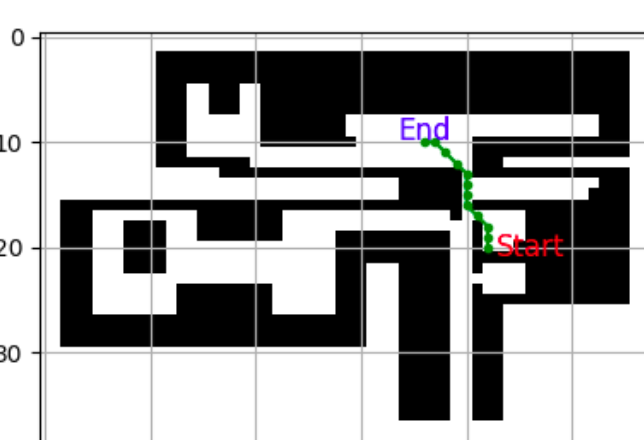
\includegraphics[scale=0.4]{figs/path1} % Escala la imagen al 150% de su tamaño original
  \caption{ Representación en el mapa del camino encontrado al primer objetivo.}
  \label{fig:vals2}
\end{figure} 

\begin{figure}[H]
  \centering
  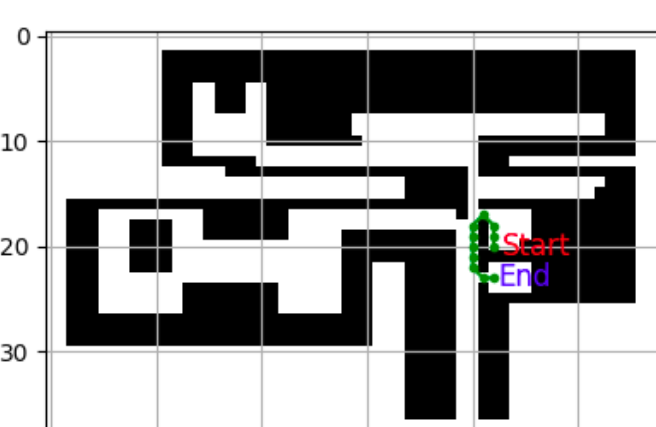
\includegraphics[scale=0.4]{figs/path2} % Escala la imagen al 150% de su tamaño original
  \caption{ Representación en el mapa del camino encontrado al segundo objetivo.}
  \label{fig:vals2}
\end{figure} 

\begin{figure}[H]
  \centering
  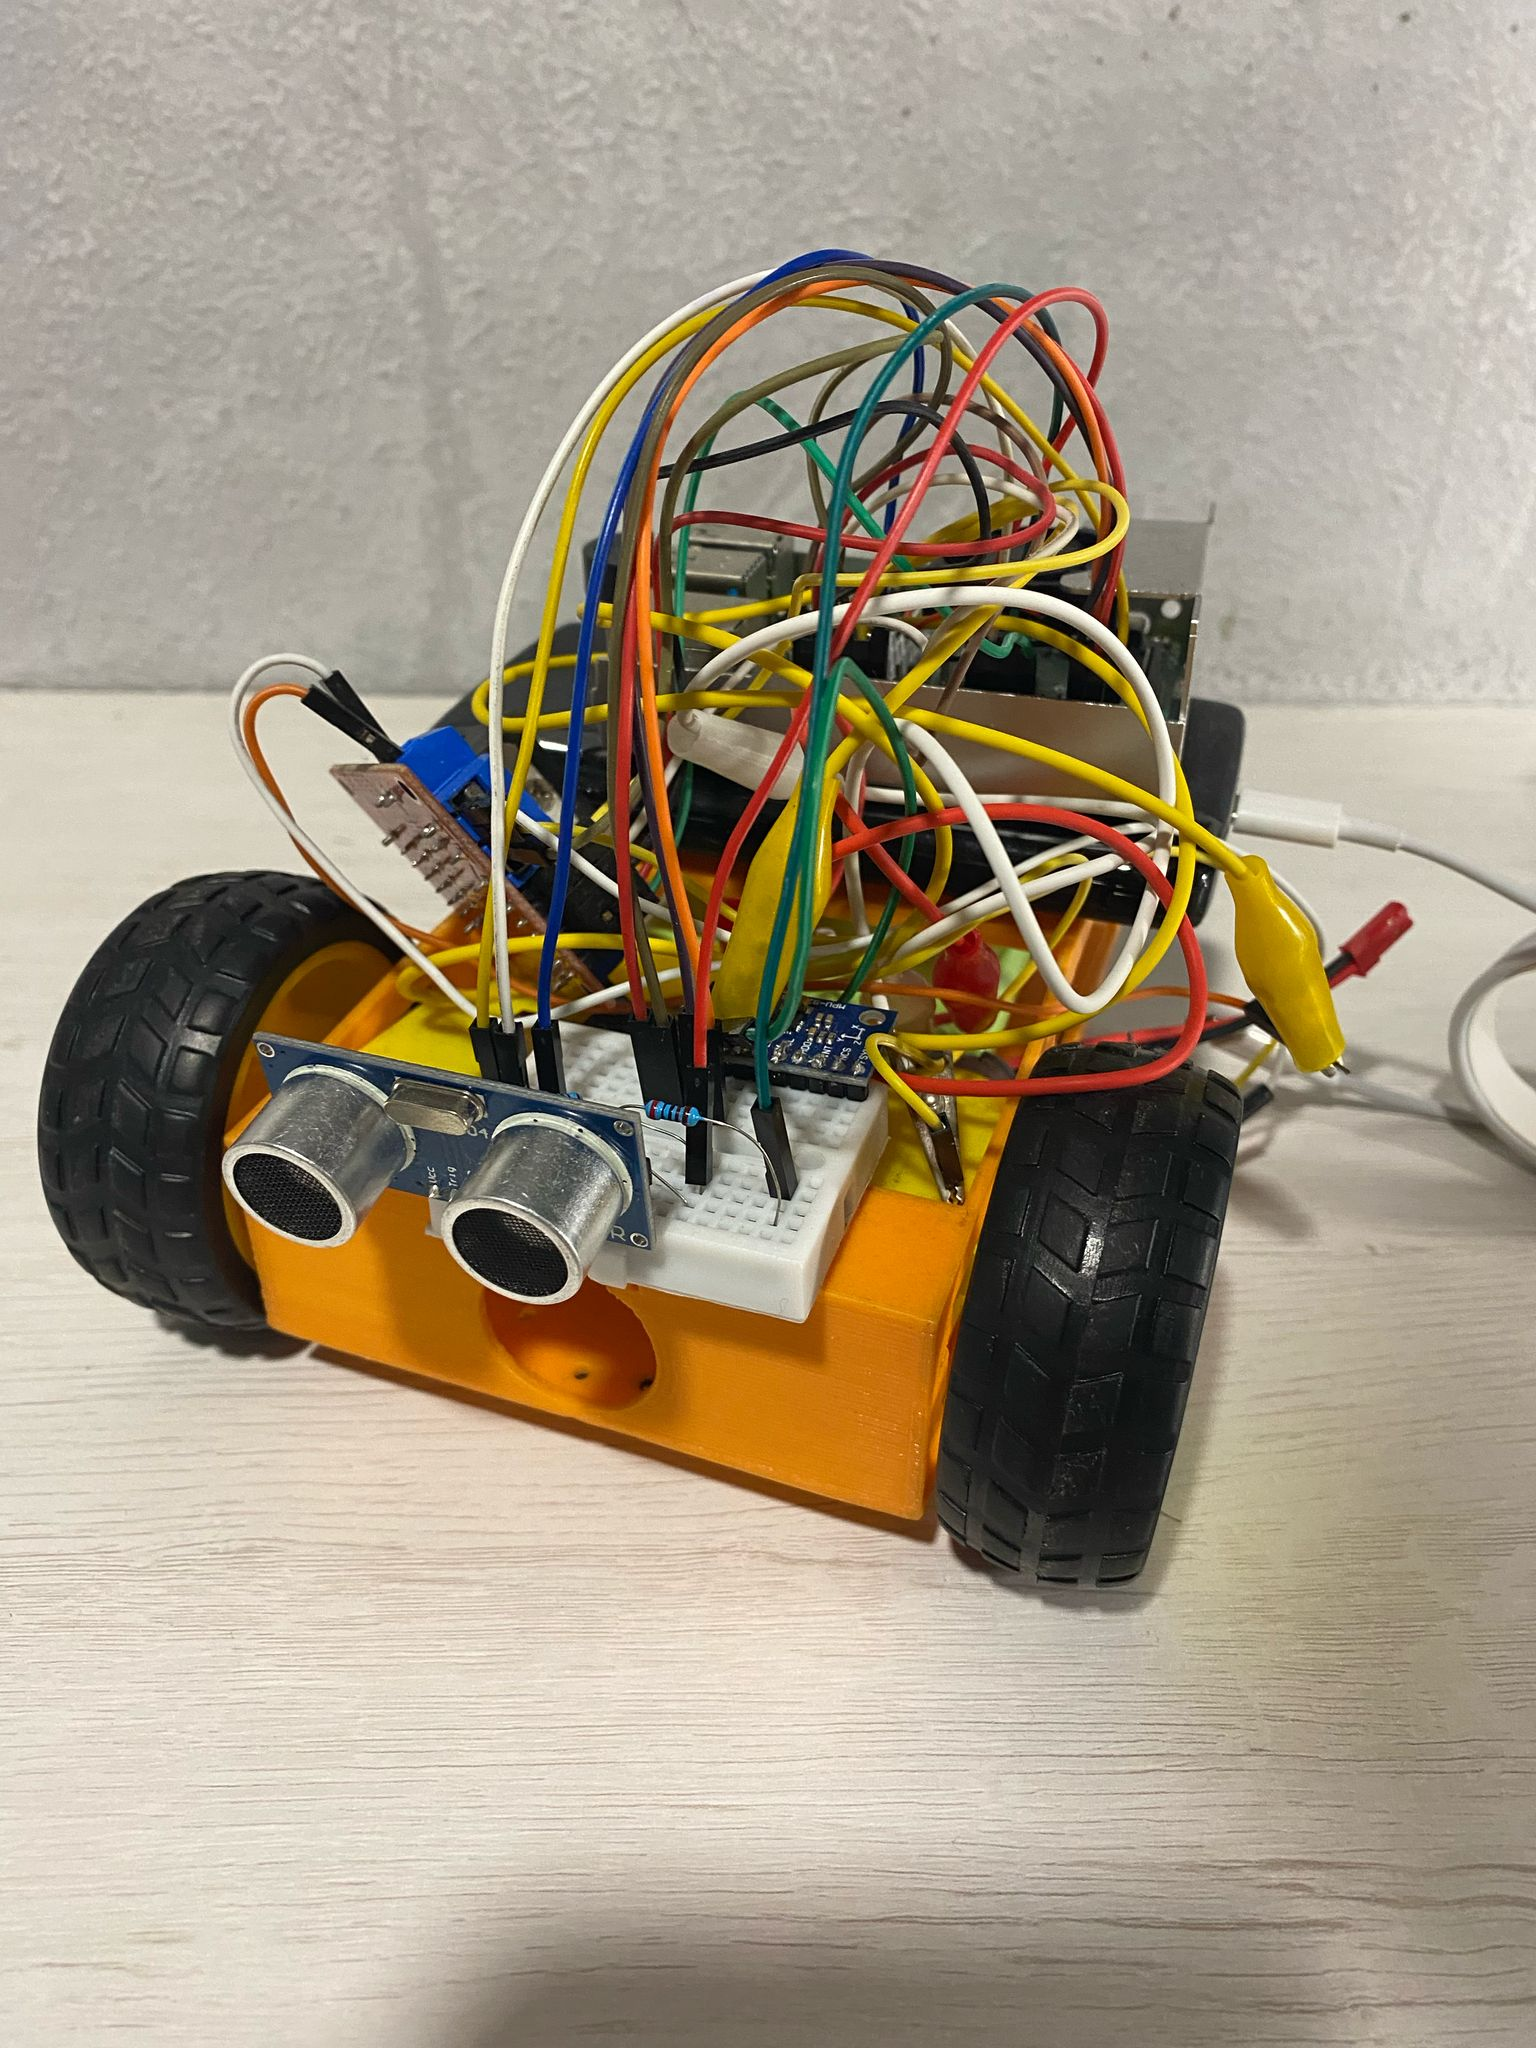
\includegraphics[scale=0.12]{figs/rob} % Escala la imagen al 150% de su tamaño original
  \caption{ Prototipo del robot final.}
  \label{fig:vals2}
\end{figure} 










